%=============================================================================
%  POSTER — PROBABILITY & STATISTICS CONFERENCE (English version)
%  Application of Multivariate Statistical Analysis in Risk Prediction and
%  Efficacy Evaluation of Plasma Exchange in Hypertriglyceridemia-Induced
%  Acute Pancreatitis
%
%  Compile with pdfLaTeX (MiKTeX/TeX Live), as in the conference template.
%  XeLaTeX/LuaLaTeX also work (fontspec branch below).
%  Figures: figs_en/ , regenerate with:  python make_figures.py en
%
%  NOTE: in baposter a LARGER fontscale means SMALLER type (the page is set at
%  fontscale * papersize and then magnified). The template ships 0.30.
%=============================================================================
\documentclass[a0paper, portrait, final, fontscale=0.40]{baposter}

\usepackage{iftex}
\ifPDFTeX
  \usepackage[utf8]{inputenc}
  \usepackage[T1]{fontenc}
  \usepackage{palatino}
\else
  \usepackage{fontspec}
  \setmainfont{texgyrepagella}[Extension=.otf, UprightFont=*-regular,
    BoldFont=*-bold, ItalicFont=*-italic, BoldItalicFont=*-bolditalic]
\fi
\usepackage[english]{babel}

\usepackage{graphicx,calc}
\usepackage{amsmath,amssymb}
\usepackage{relsize}
\usepackage{multirow,multicol}
\usepackage{rotating,enumerate,floatflt}
\usepackage{bm,url,booktabs}

\newcommand{\captionfont}{\footnotesize}
\graphicspath{{figs_en/}{images/}{../images/}}
\usetikzlibrary{calc}

\setlength{\columnsep}{1.0em}
\setlength{\columnseprule}{0mm}

\newcommand{\compresslist}{%
	\setlength{\itemsep}{1pt}%
	\setlength{\parskip}{0pt}%
	\setlength{\parsep}{0pt}%
}

% ---- Palette: contrast- and CVD-checked -----------------------------------
\definecolor{boxblue}{RGB}{0, 71, 146}
\definecolor{cviolet}{RGB}{58, 45, 132}
\definecolor{cteal}{RGB}{13, 110, 84}
\definecolor{corange}{RGB}{176, 70, 25}
\definecolor{cmagenta}{RGB}{154, 44, 85}
\definecolor{cgreen}{RGB}{11, 92, 45}
\definecolor{cgrey}{RGB}{82, 81, 78}
\definecolor{lblue}{RGB}{233, 240, 251}
\definecolor{lteal}{RGB}{229, 246, 240}
\definecolor{lorange}{RGB}{253, 238, 230}
\definecolor{lmagenta}{RGB}{252, 236, 242}
\definecolor{lgreen}{RGB}{232, 245, 235}
\definecolor{alb}{RGB}{42, 120, 214}
\definecolor{ffp}{RGB}{235, 104, 52}
\definecolor{sigred}{RGB}{199, 42, 41}

\newcommand{\hl}[1]{\textcolor{cviolet}{\textbf{#1}}}
\newcommand{\key}[1]{\textbf{\textcolor{sigred}{#1}}}
\newcommand{\shead}[2]{\textcolor{#2}{\textbf{#1}}}

\begin{document}

	\begin{poster}%
	{
		grid=false,
		colspacing=0.7em,
		headerColorOne = boxblue,
		borderColor=boxblue,
		textborder=faded,
		headerborder=open,
		headerfont = \color{white}\bfseries\Large,
		headershape=roundedright,
		headershade=plain,
		background=none,
		bgColorOne=white,
		boxshade=plain,
		boxColorOne=white,
		headerheight=0.078\textheight
	}
	{
\includegraphics[height = 8.3em]{Logo Đơn.png}}
	{\vspace{0.15em}
	 \LARGE \textbf{Application of Multivariate Statistical Analysis in Risk Prediction and Efficacy}\\[0.25em]
	 \LARGE \textbf{Evaluation of Plasma Exchange in Hypertriglyceridemia-Induced Acute Pancreatitis}\vspace{0.25em}}
	{ \Large Phan Thai Son$^{1}$, \ Pham Hieu Dan$^{2}$, \ Nguyen Minh Toan$^{3}$, \
	  Luu Phuc Loi$^{2}$, \ Hoang Van Quang$^{2,*}$ \\[0.15em]
	  \normalsize $^{1}$University Medical Center HCMC \ $\cdot$ \ $^{2}$Thong Nhat Hospital
	  \ $\cdot$ \ $^{3}$School of Pharmacy, UMP-HCMC \ $\cdot$ \ $^{*}$corresponding author}
	{
\includegraphics[height = 8.0em]{LOGO KHOA - ĐỨNG - KHÔNG NỀN.png}}

	%=========================================================================
	% ROW 1 — CLINICAL BACKGROUND + STUDY DESIGN  |  ANALYSIS PIPELINE
	%=========================================================================
	\headerbox{\ \ Clinical background and objective}%
		{name=clinical,column=0,row=0,
		 headerColorOne=boxblue,borderColor=boxblue}{
		{\small
		\shead{Why HTG-induced pancreatitis matters.}{boxblue}
		Hypertriglyceridemia (HTG) is the third most common cause of acute pancreatitis after
		gallstones and alcohol, and proportionally more frequent in Asian cohorts. Once
		serum triglyceride (TG) passes \textbf{1000 mg/dL} ($11.3$ mmol/L), chylomicrons
		obstruct the pancreatic microcirculation and lipase-released free fatty acids injure
		acinar cells. HTG-AP runs a more severe course than other aetiologies, so the aim is to
		bring TG below $500$--$1000$ mg/dL \emph{as fast as possible}.\\[0.4em]
		\shead{Why the replacement fluid is an open question.}{boxblue}
		Plasma exchange (TPE) removes chylomicrons directly, but ASFA grades HTG-AP only as
		\textbf{Category III, Grade 2C}~[1]: the evidence establishes neither which patients
		benefit nor which fluid to use. \textcolor{ffp}{\textbf{Fresh frozen plasma}} restores
		lipoprotein lipase but carries transfusion reactions, citrate load and cost;
		\textcolor{alb}{\textbf{5\% albumin}} avoids all three. The choice is made at the
		bedside, \emph{not} by protocol.\\[0.4em]
		\shead{Objective.}{cviolet}
		\emph{Who deteriorates}, \emph{does TPE work}, \emph{does the fluid matter} --- mapping
		onto risk prediction, paired pre--post measurement and group comparison under
		non-random allocation. With only \key{15 events} and \key{33 parallel tests},
		\hl{type I error control} and \hl{sensitivity checking} separate a real effect from an
		apparent one.}
	}

	\headerbox{\ \ Study design}{name=design,column=1,row=0,
		headerColorOne=cteal,borderColor=cteal}{
		\centering
		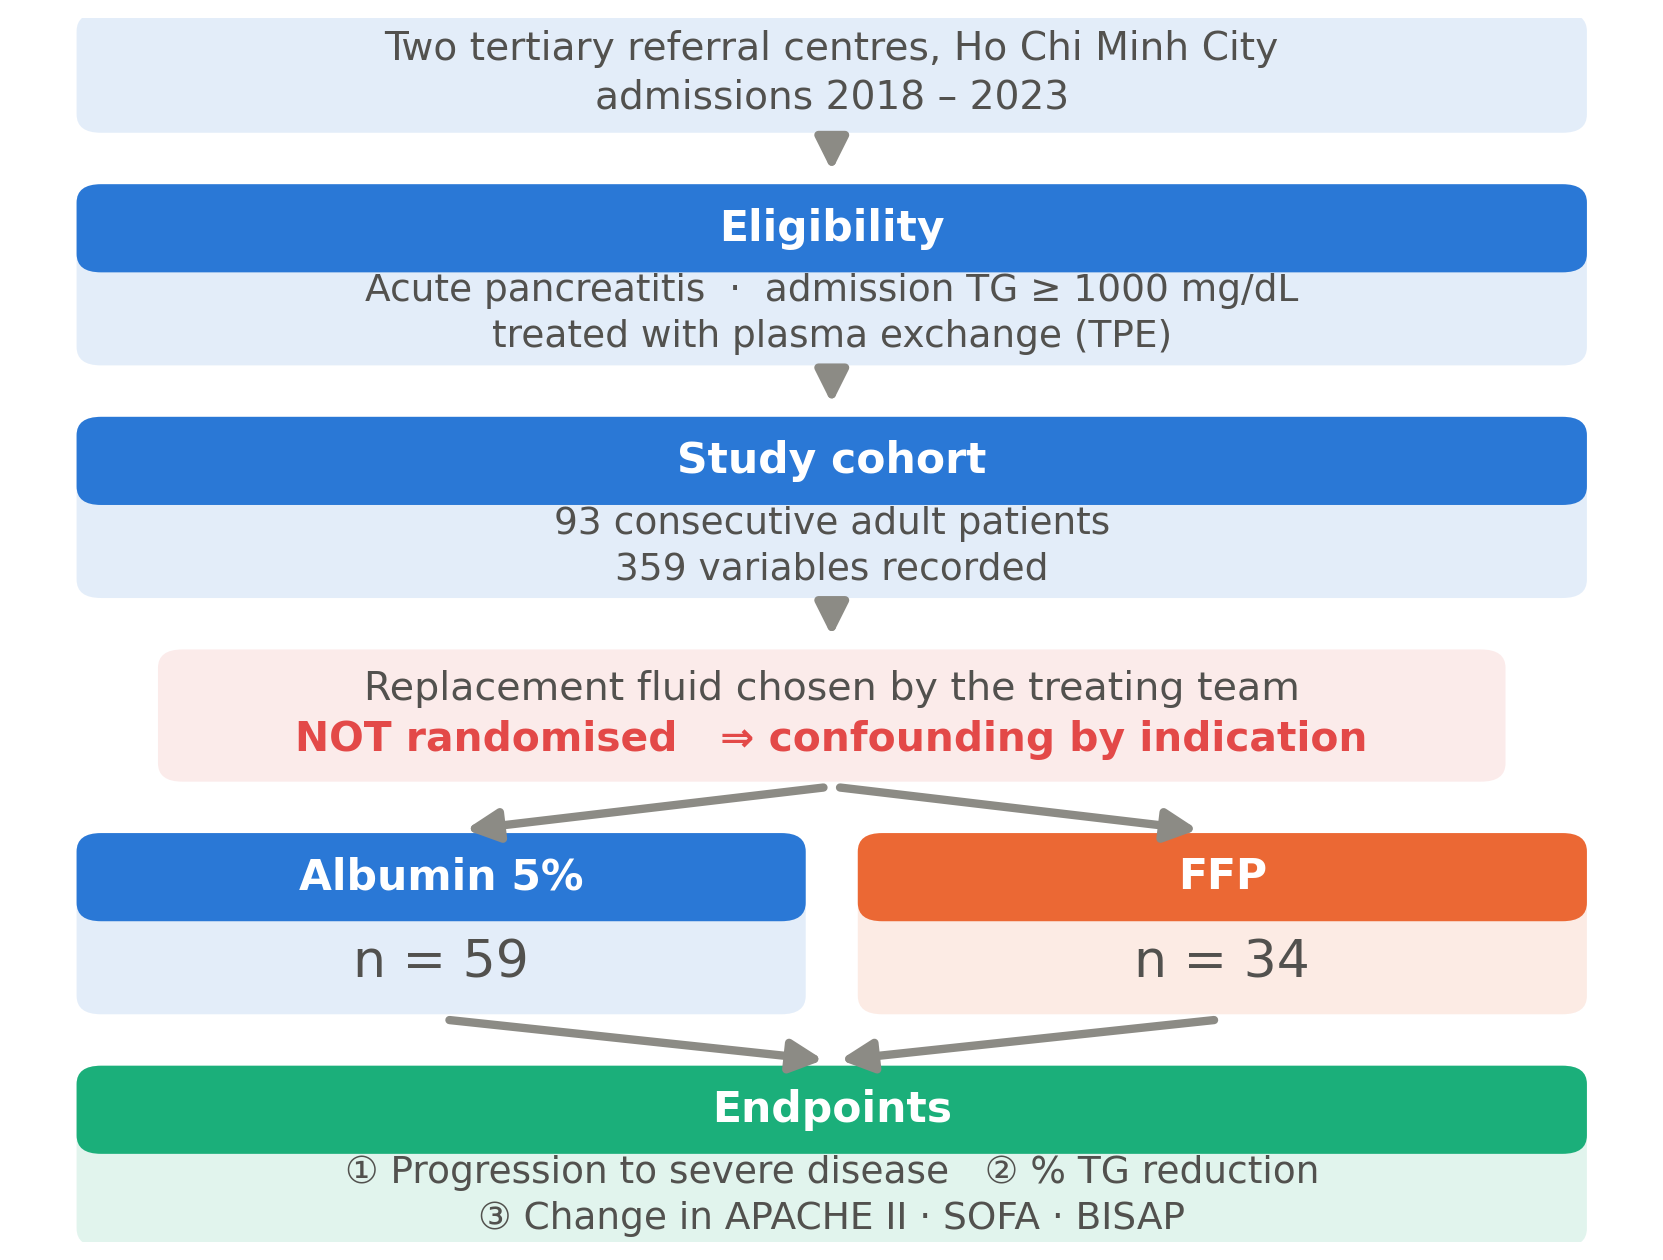
\includegraphics[width=\linewidth]{f00_study_design.png}
		\par\vspace{0.25em}
		{\scriptsize\textcolor{cgrey}{Patient flow. The branch point is the whole statistical
		difficulty: allocation was clinical, not random.}}
	}

	\headerbox{\ \ Statistical analysis pipeline}{name=method,column=2,row=0,
		headerColorOne=cviolet,borderColor=cviolet}{
		\centering
		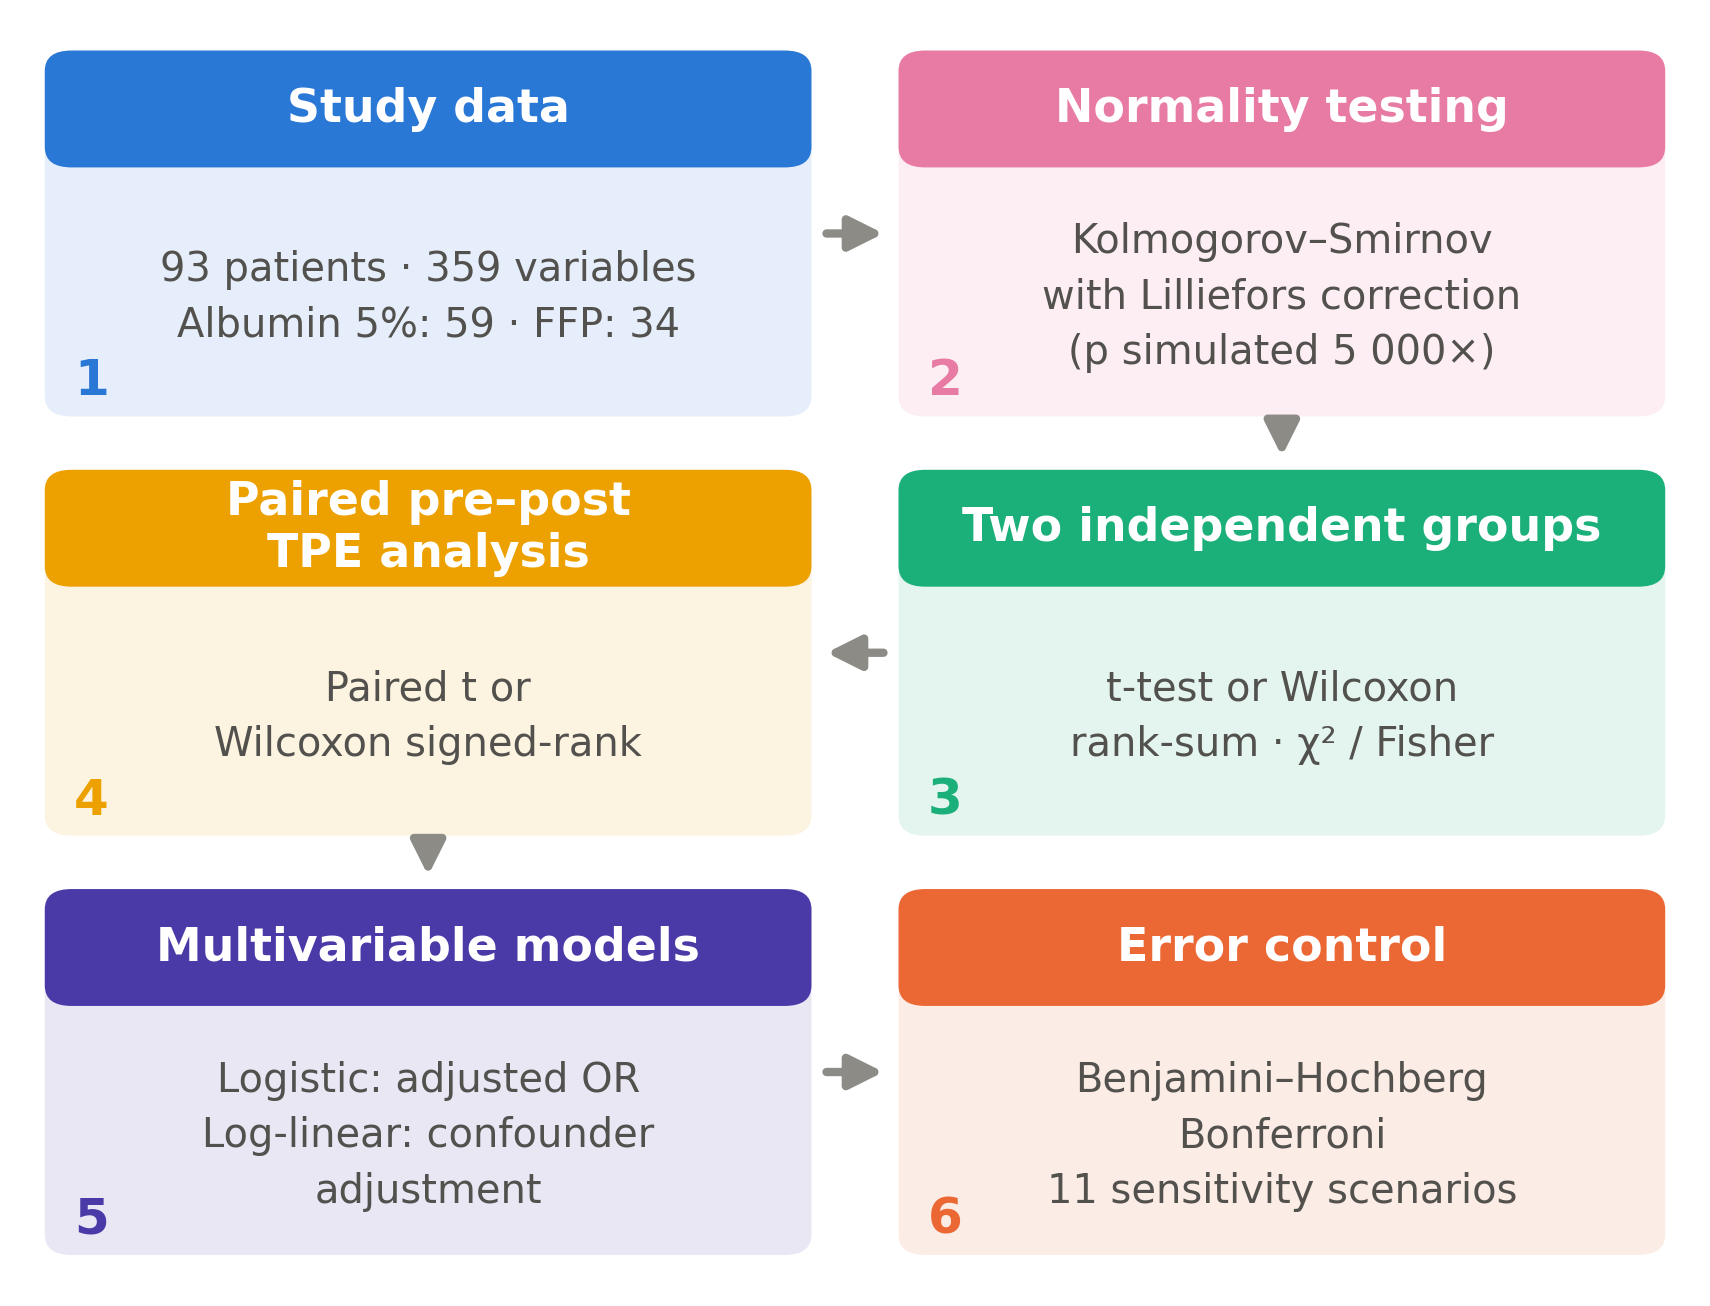
\includegraphics[width=\linewidth]{f0_pipeline_tall.png}
		\par\vspace{0.25em}
		{\scriptsize\textcolor{cgrey}{Tests follow from the normality result in step 2; steps 5
		and 6 exist to keep false positives out of the conclusion.}}
	}

	%=========================================================================
	% ROW 2 — RESULT 1
	%=========================================================================
	\headerbox{\ \ Result 1 --- Distribution drives test choice \ $\cdot$ \ Univariate analysis of severity}%
		{name=kq1,column=0,span=3,row=0,below=design,
		 headerColorOne=cteal,borderColor=cteal}{

		\begin{minipage}[b]{0.505\linewidth}\vspace{0pt}
		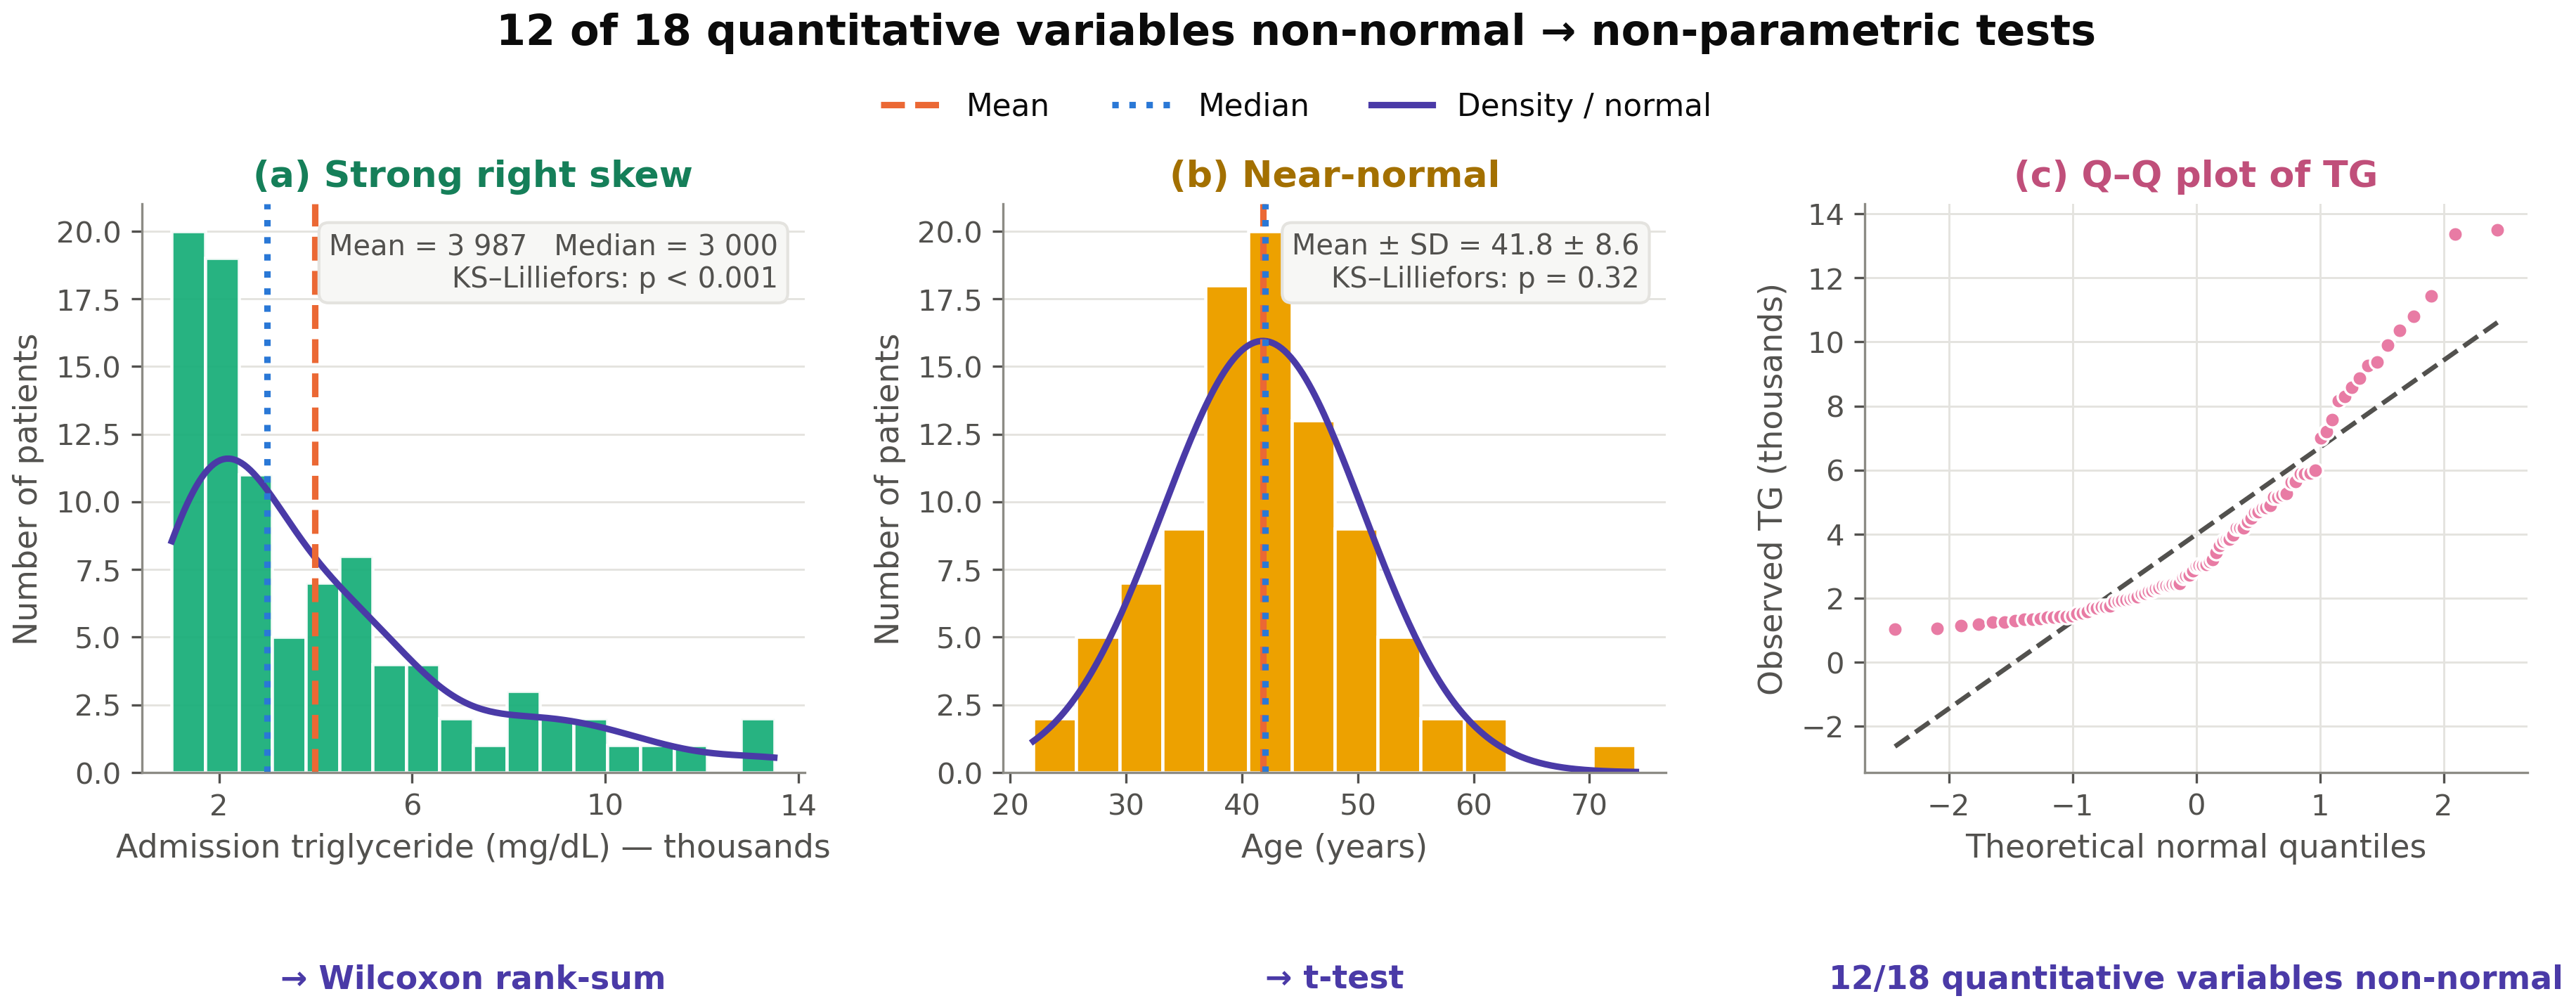
\includegraphics[width=\linewidth]{f1_distribution.png}
		\end{minipage}%
		\hfill
		\begin{minipage}[b]{0.480\linewidth}\vspace{0pt}
		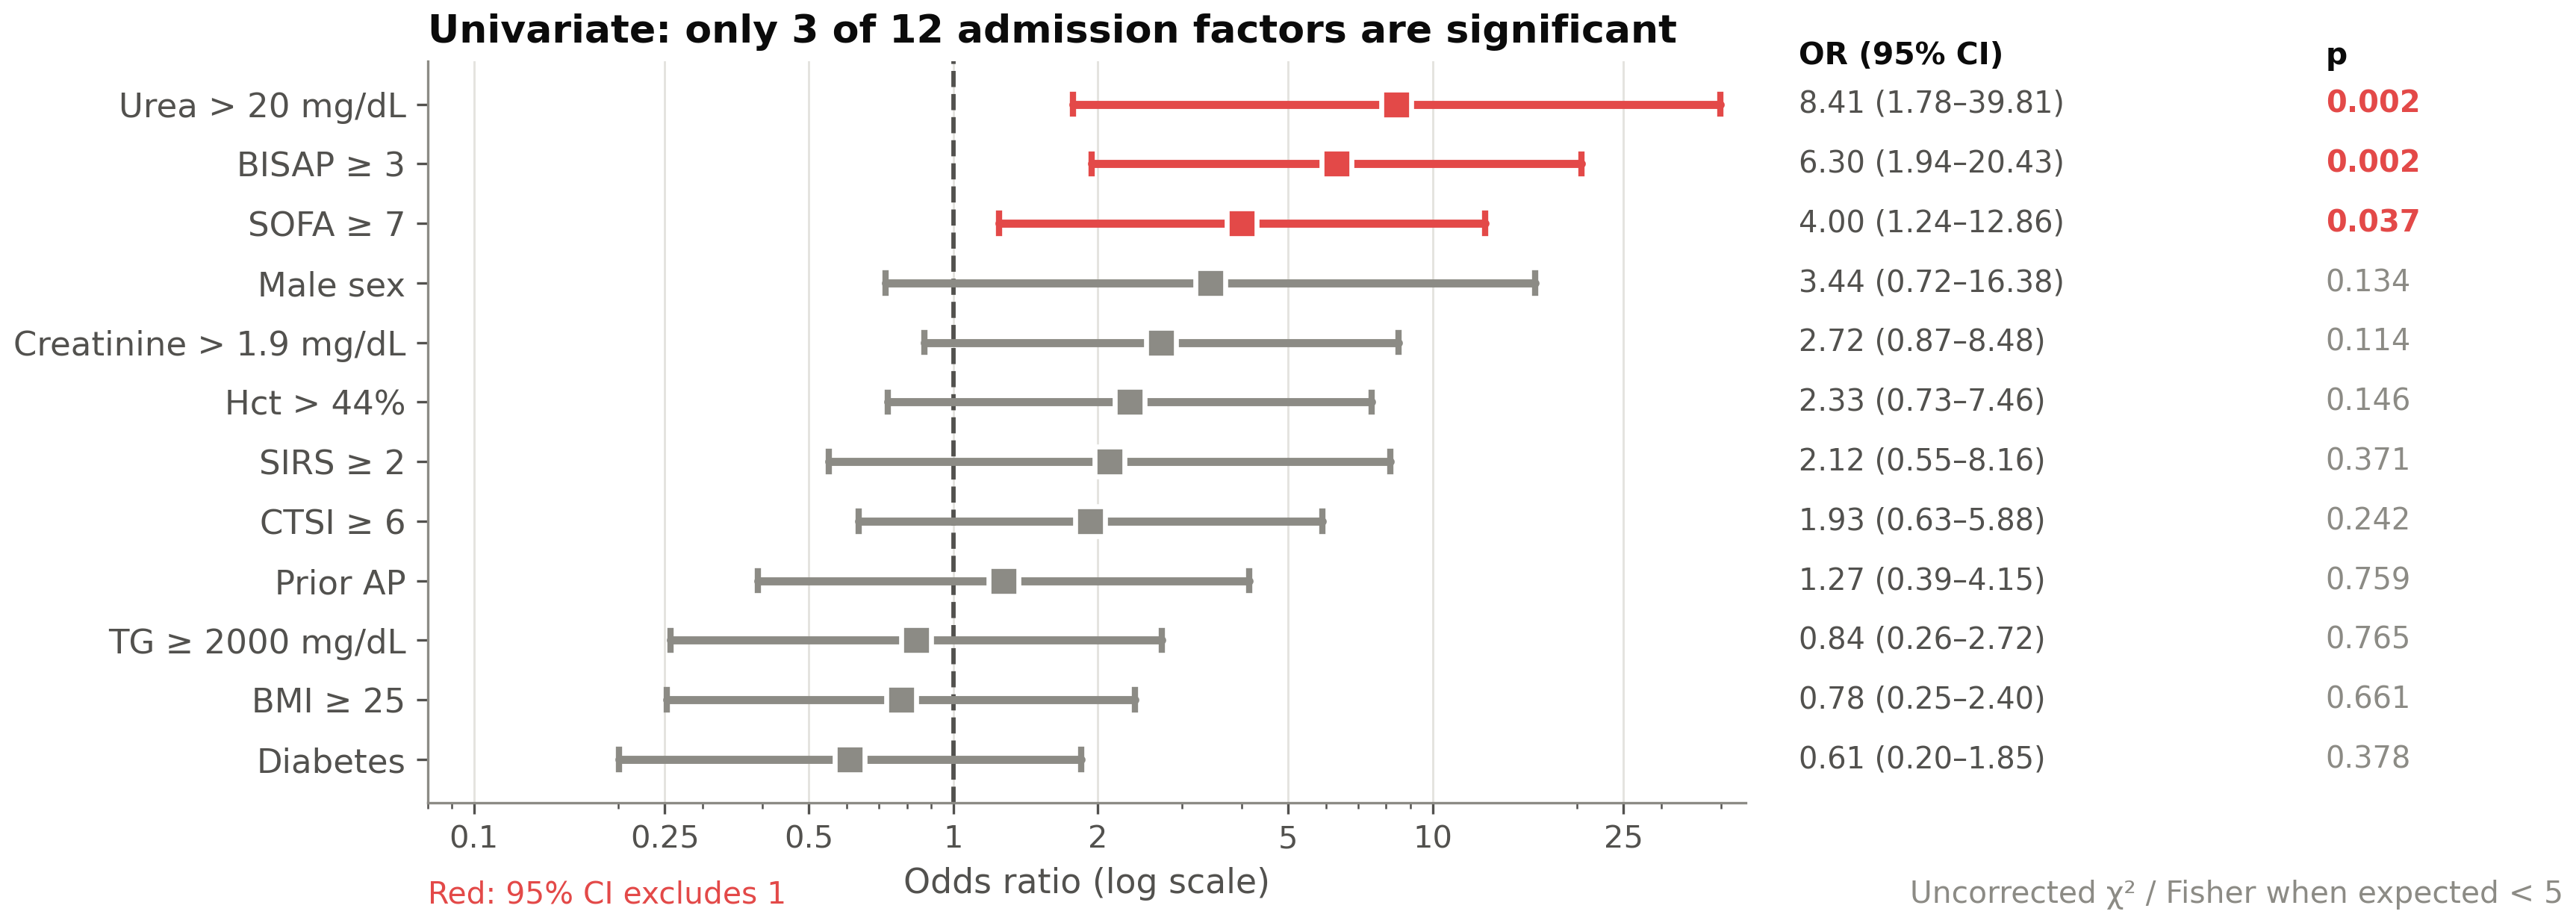
\includegraphics[width=\linewidth]{f3_forest_univariate.png}
		\end{minipage}

		\vspace{0.2em}
		{\small \textcolor{cteal}{$\blacktriangleright$} \
		\textbf{12 of 18} quantitative variables are non-normal, so non-parametric tests are the
		default. Three factors have a 95\% CI excluding 1, all with very wide intervals ---
		a direct consequence of 15 events. \key{Caveat:} the severity proxy shares its components
		with BISAP and SIRS, so part of this association is \textbf{definitional}.}
	}

	%=========================================================================
	% ROW 3 — RESULT 2
	%=========================================================================
	\headerbox{\ \ Result 2 --- Multivariable logistic regression \ $\cdot$ \ Efficacy of plasma exchange (paired)}%
		{name=kq2,column=0,span=3,row=0,below=kq1,
		 headerColorOne=corange,borderColor=corange}{

		\begin{minipage}[b]{0.443\linewidth}\vspace{0pt}
		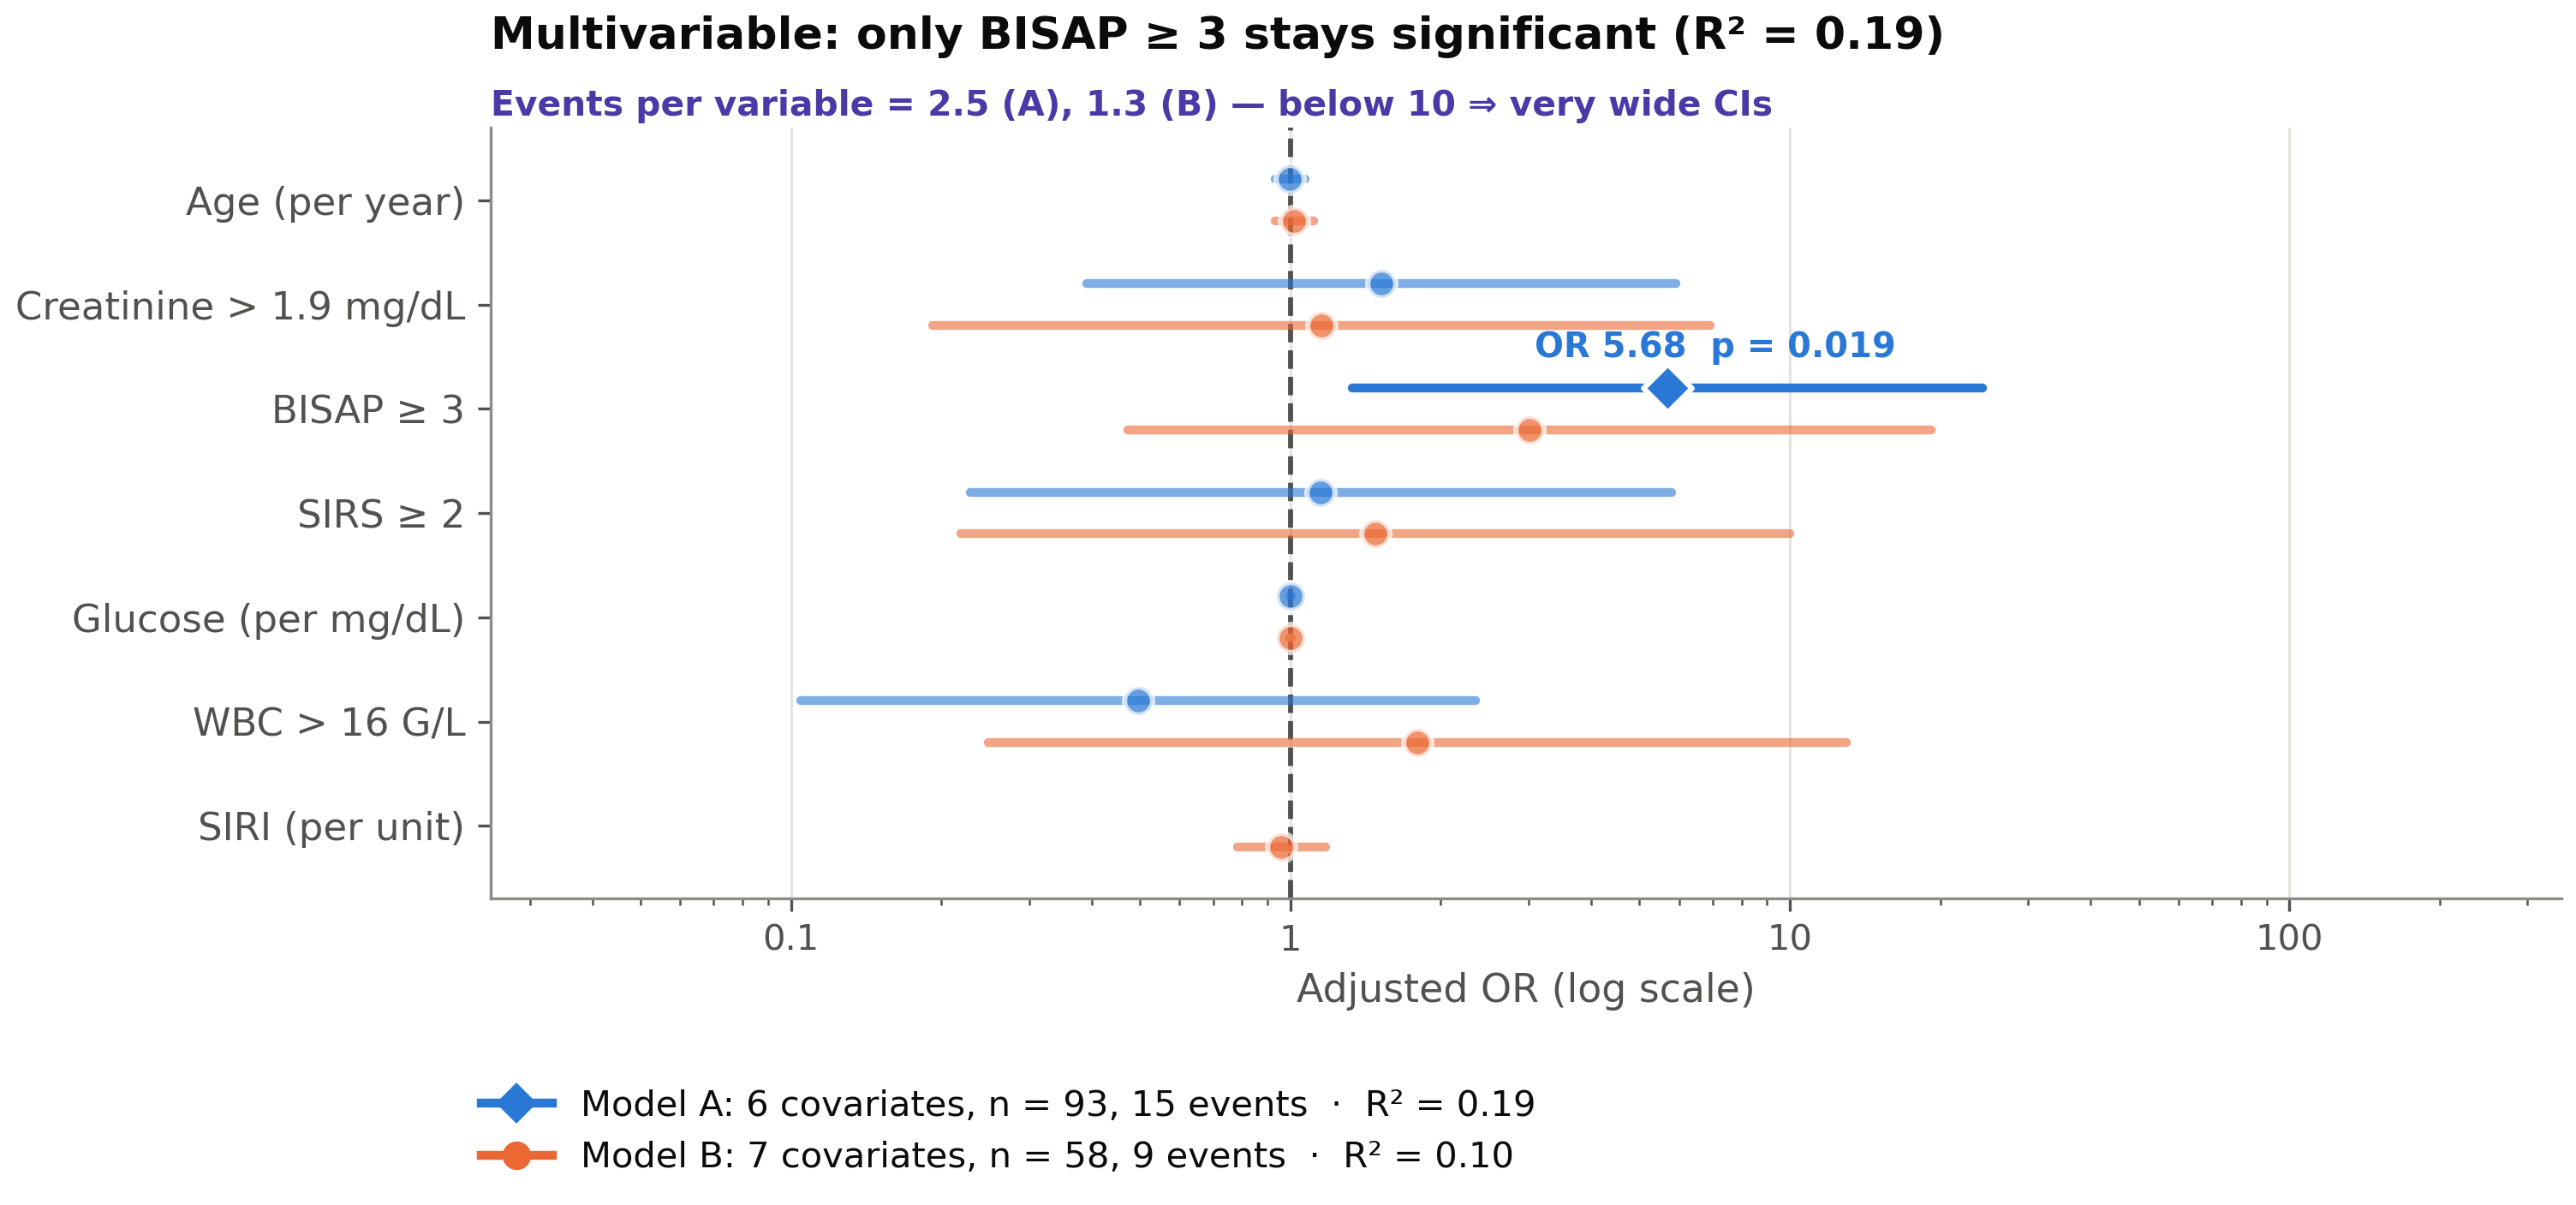
\includegraphics[width=\linewidth]{f4_forest_multivariable.png}
		\end{minipage}%
		\hfill
		\begin{minipage}[b]{0.538\linewidth}\vspace{0pt}
		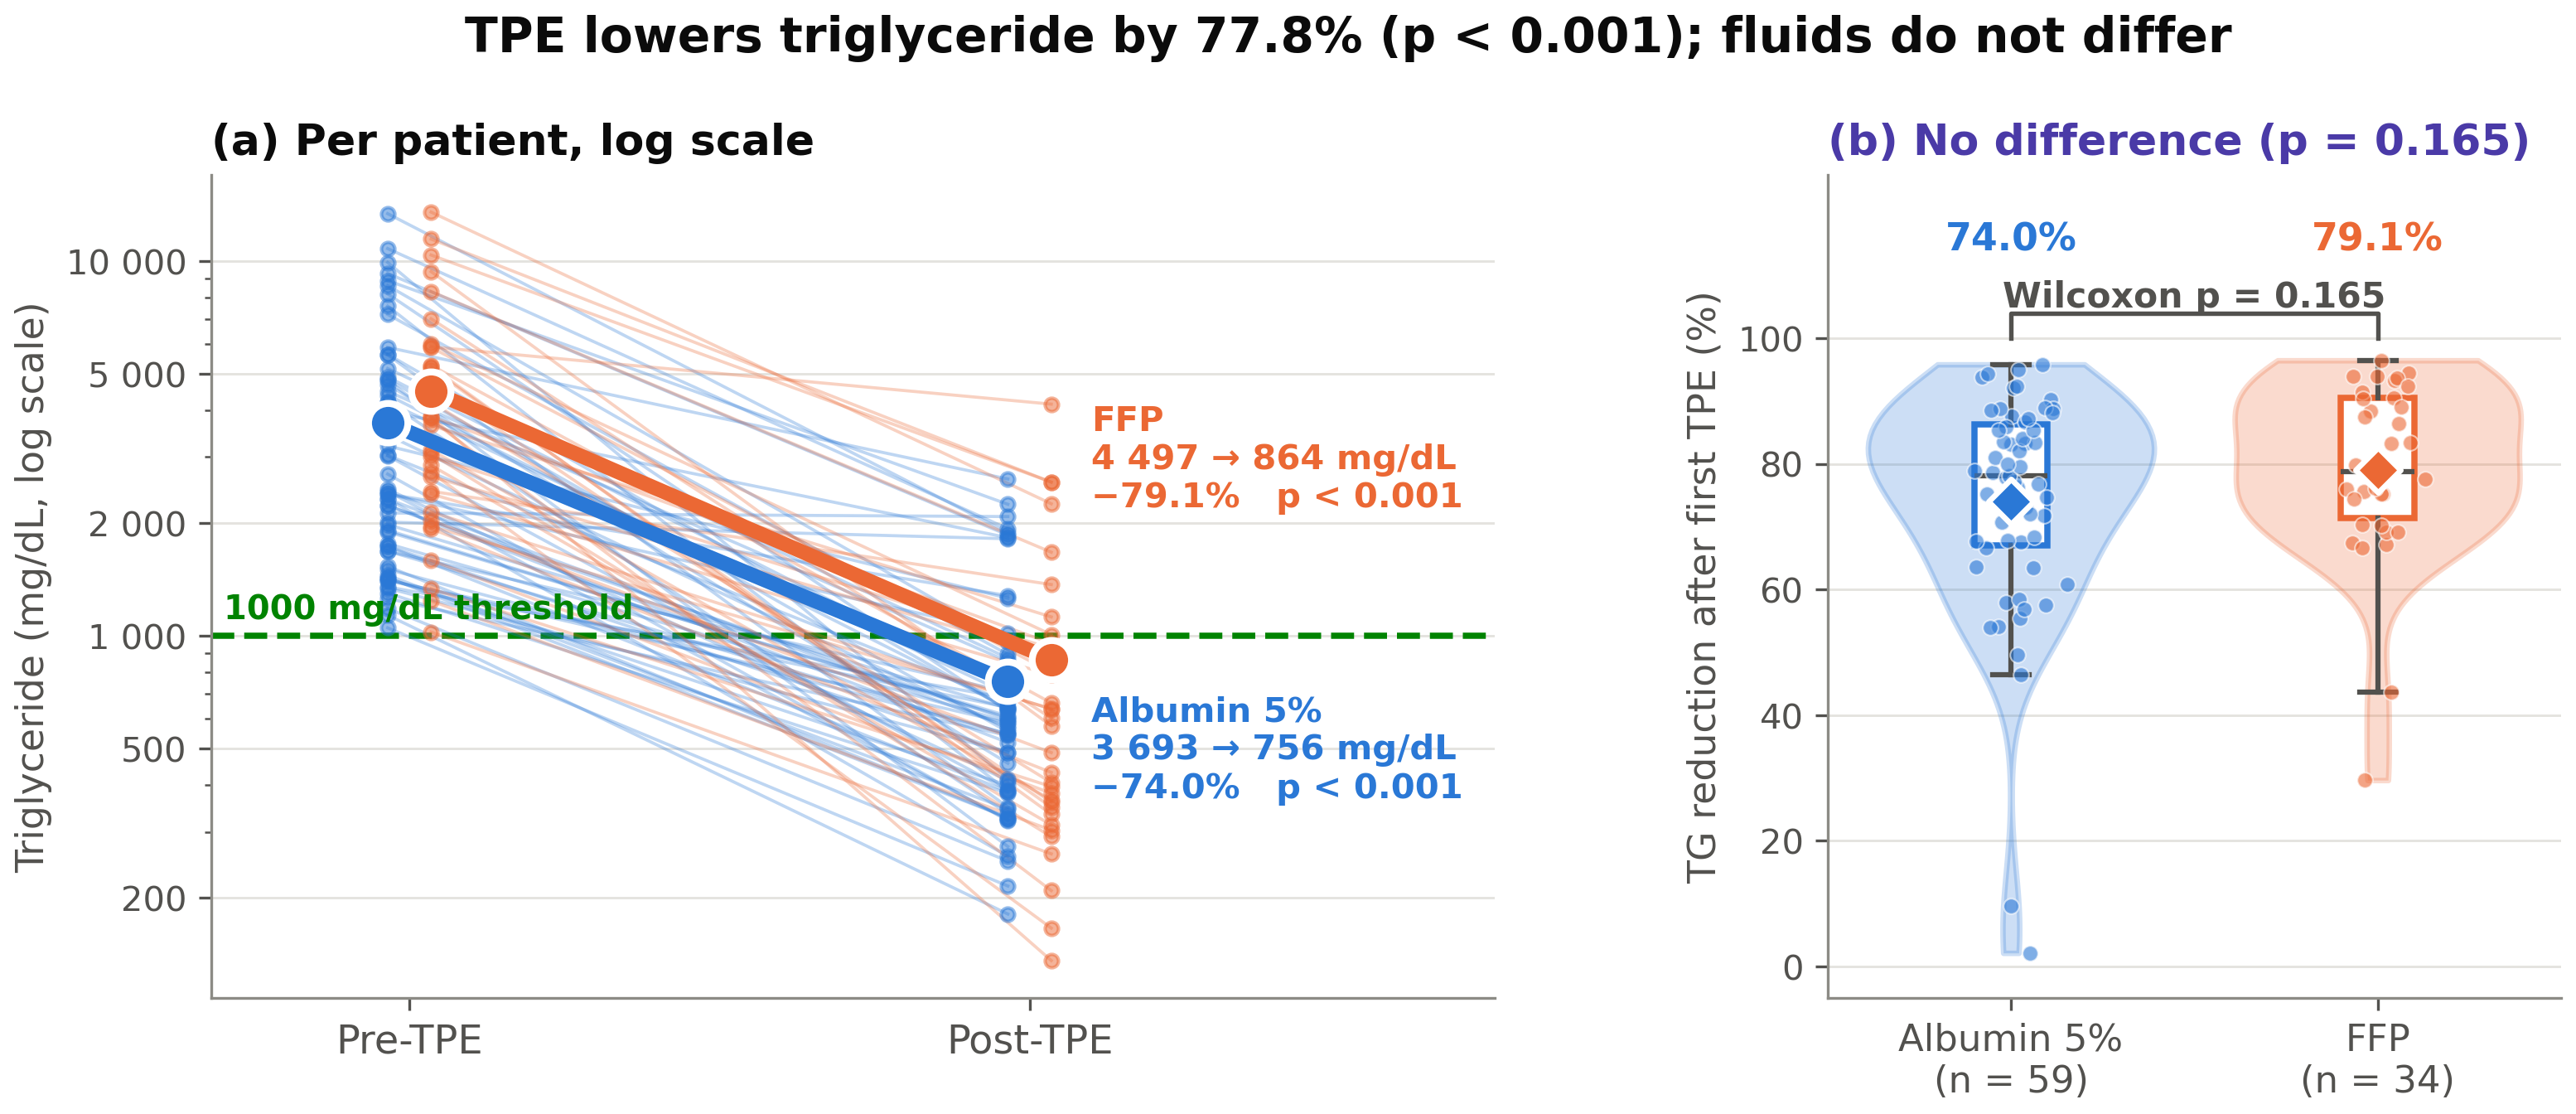
\includegraphics[width=\linewidth]{f5_paired_tg.png}
		\end{minipage}

		\vspace{0.2em}
		{\small \textcolor{corange}{$\blacktriangleright$} \
		Only BISAP $\geq3$ survives adjustment ($R^{2}=0.19$); at \key{2.5 events per covariate},
		far below the Peduzzi rule of 10, the model is \textbf{exploratory}, not a prognostic
		score. The paired analysis, by contrast, is unambiguous: TG $-77.8\%$ ($p<0.001$),
		\textbf{79.6\%} reach $<1000$ mg/dL after one session, and APACHE II, SOFA and BISAP all
		improve ($p<0.001$).}
	}

	%=========================================================================
	% ROW 4 — RESULT 3
	%=========================================================================
	\headerbox{\ \ Result 3 --- Albumin 5\% versus FFP: confounder adjustment \ $\cdot$ \ multiplicity control}%
		{name=kq3,column=0,span=3,row=0,below=kq2,
		 headerColorOne=cmagenta,borderColor=cmagenta}{

		\begin{minipage}[b]{0.464\linewidth}\vspace{0pt}
		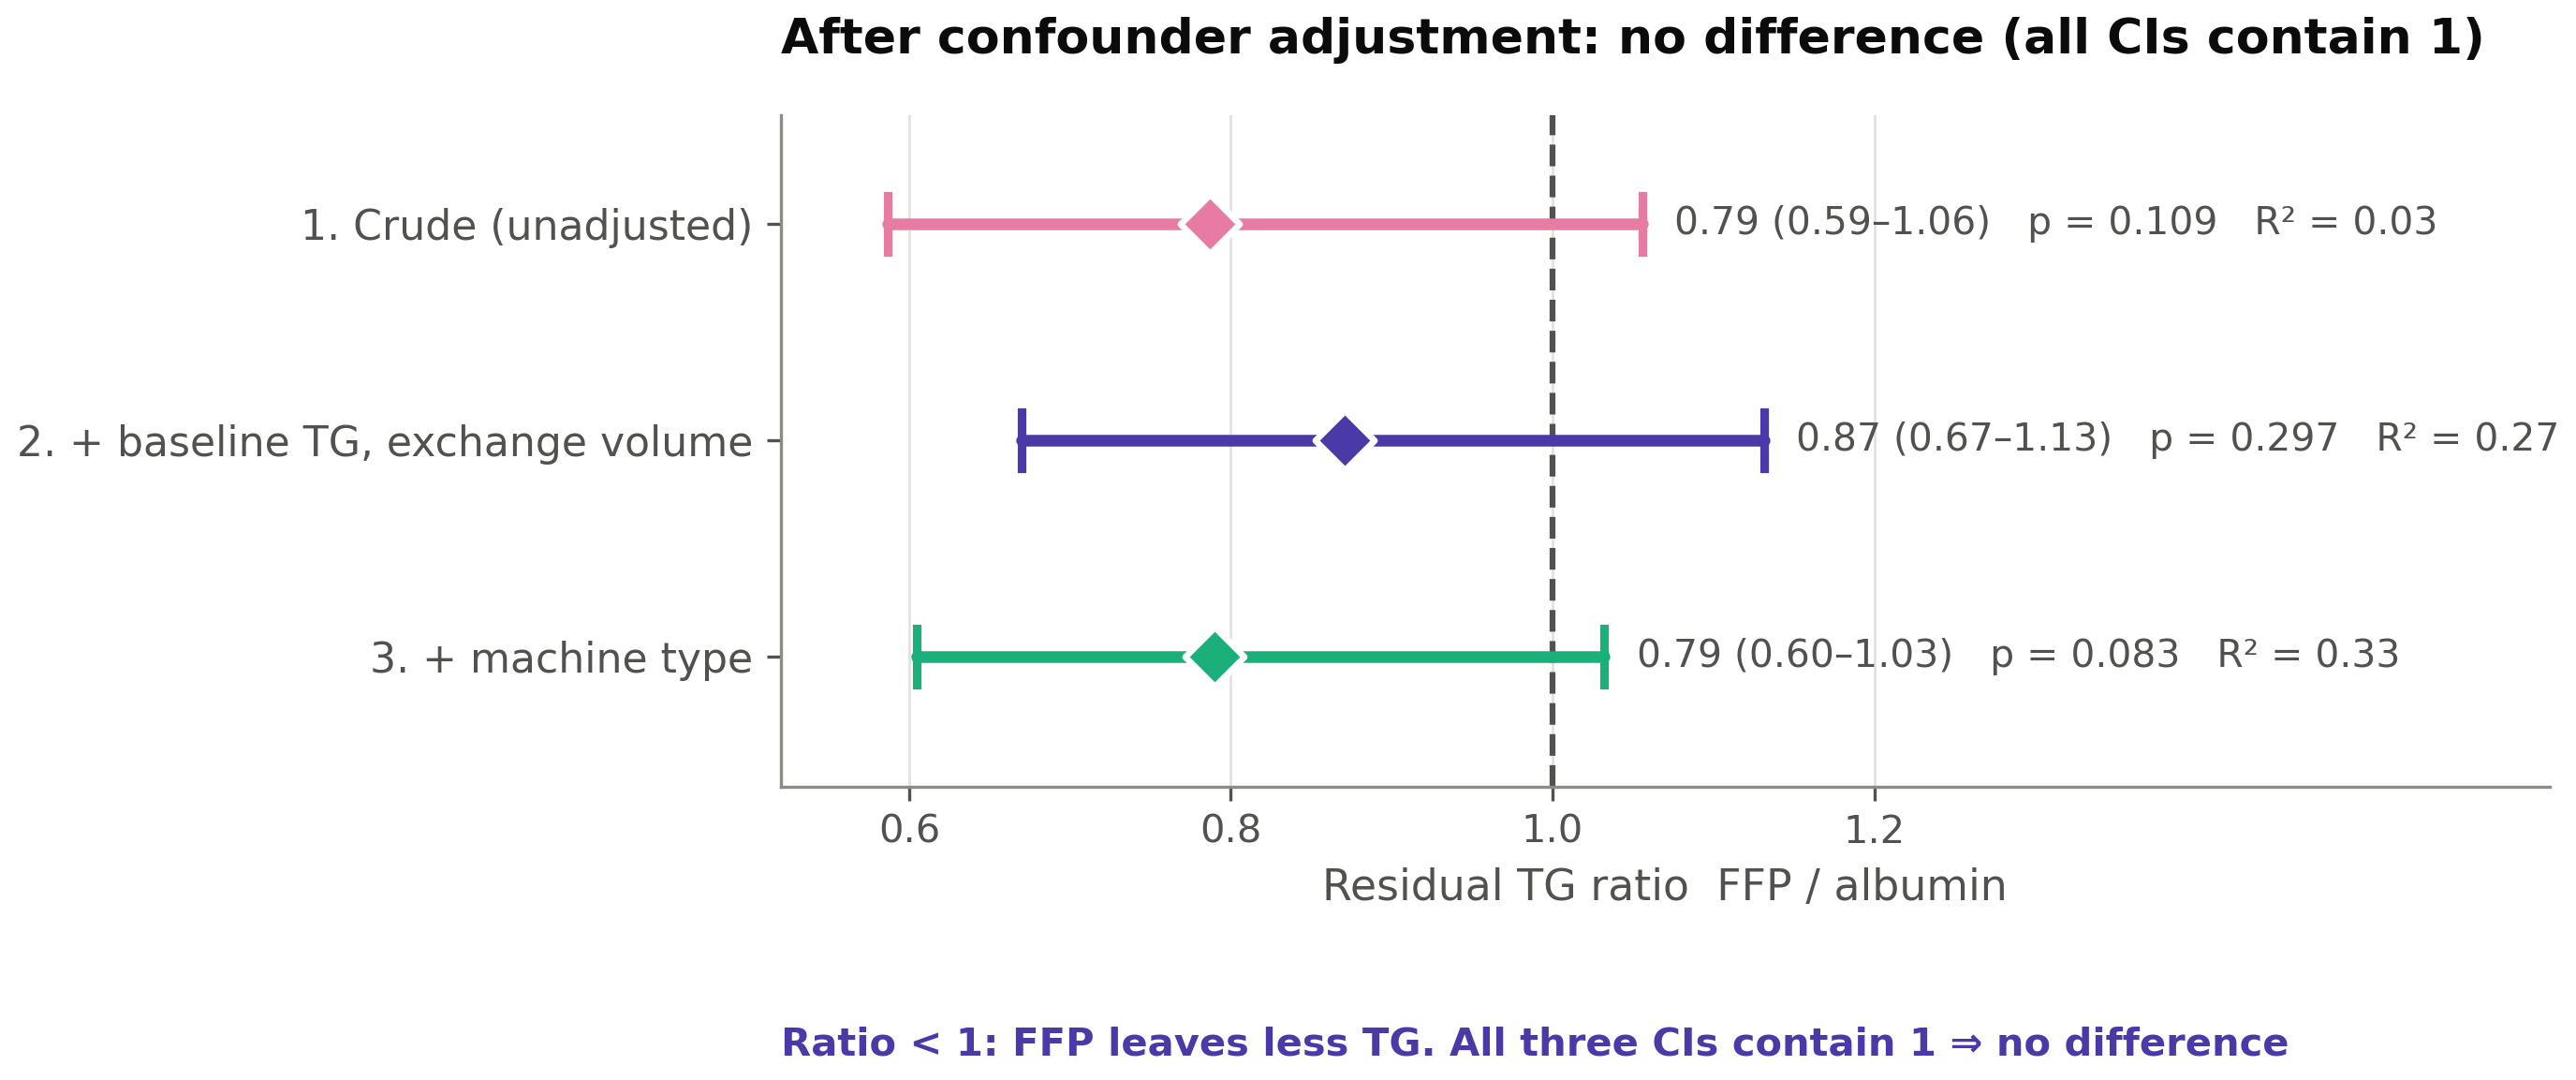
\includegraphics[width=\linewidth]{f8_adjusted.png}
		\end{minipage}%
		\hfill
		\begin{minipage}[b]{0.510\linewidth}\vspace{0pt}
		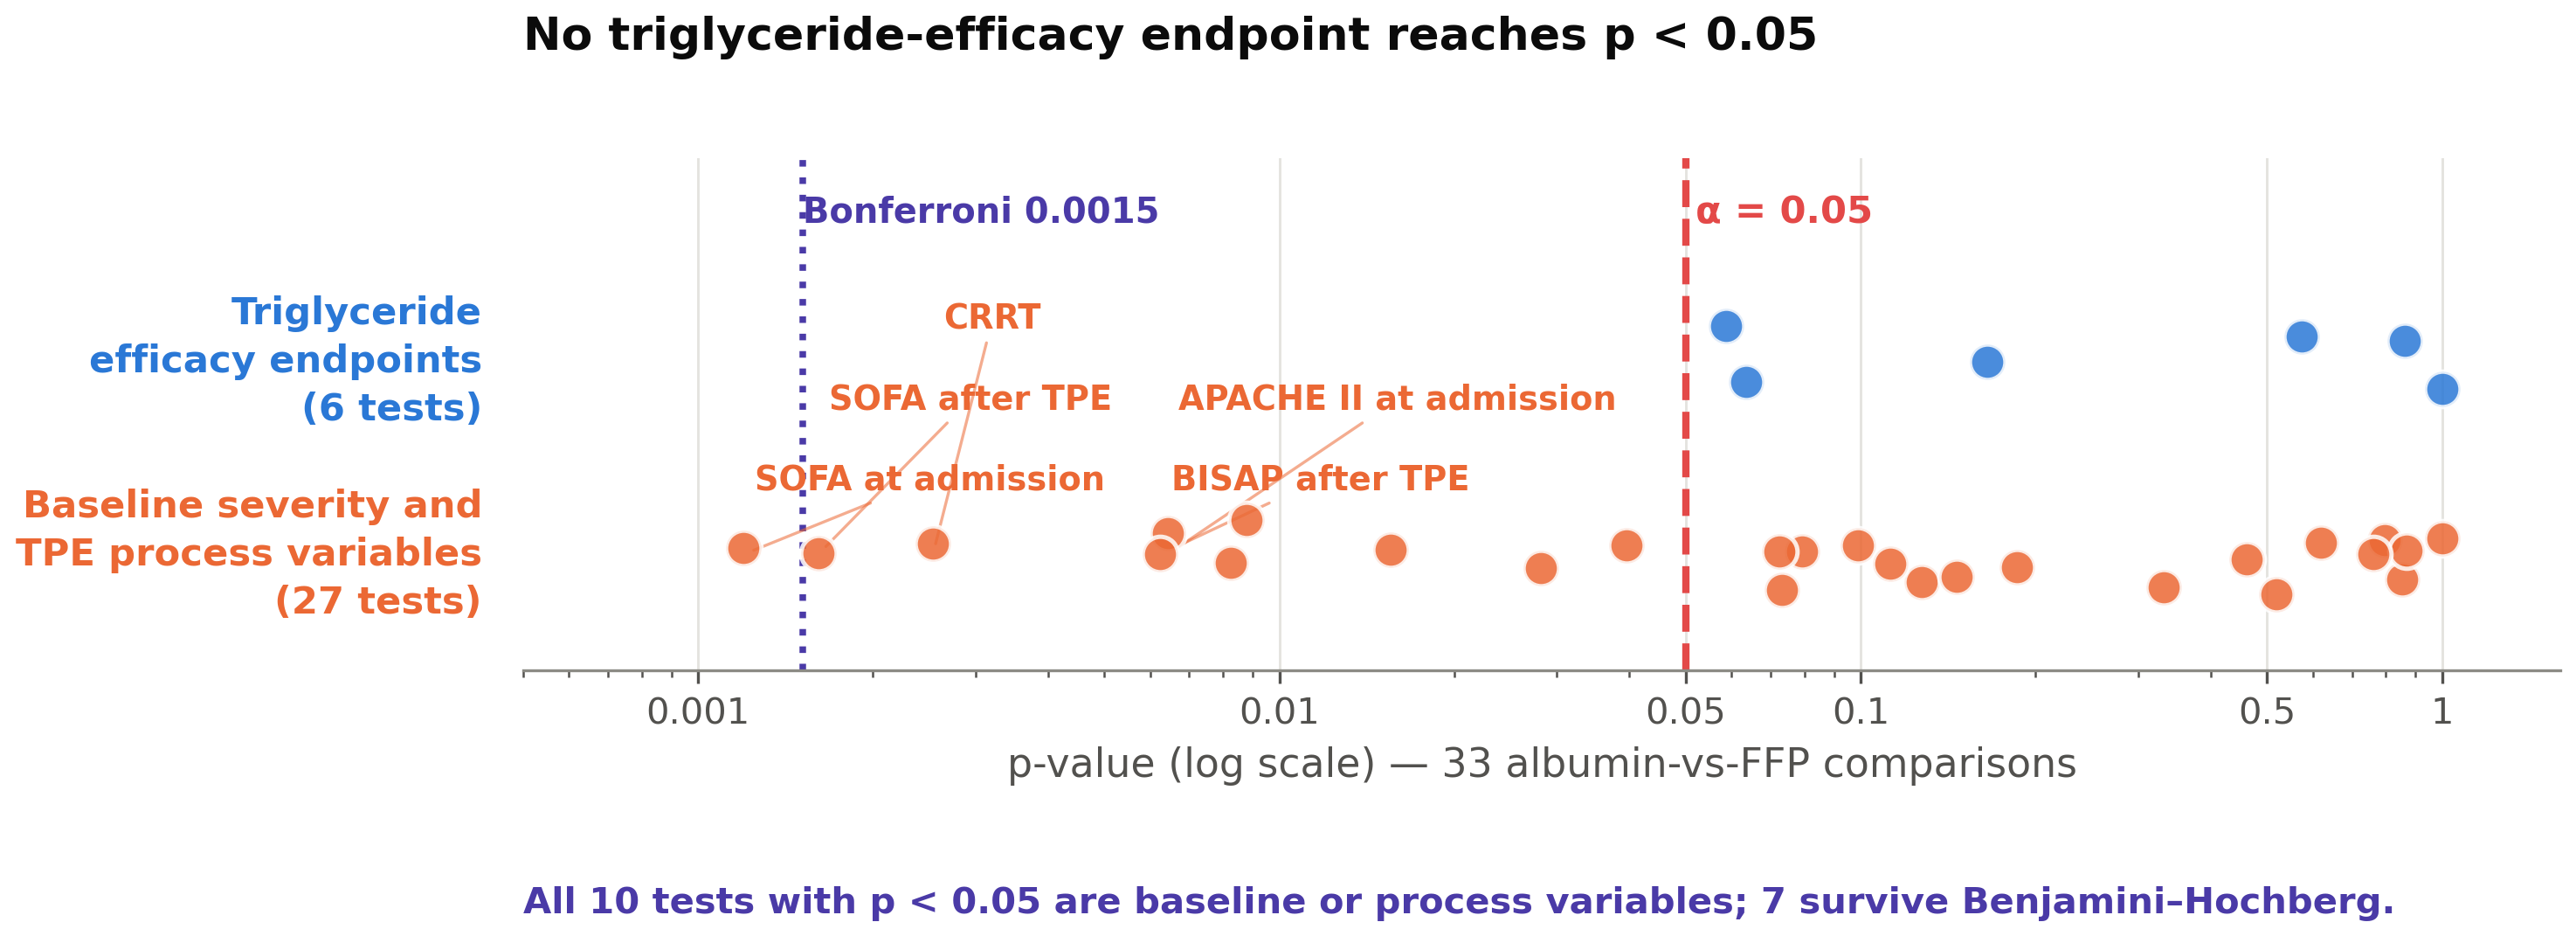
\includegraphics[width=\linewidth]{f9_pvalue_strip.png}
		\end{minipage}

		\vspace{0.2em}
		{\small \textcolor{cmagenta}{$\blacktriangleright$} \
		The FFP group was \emph{sicker from the outset} (SOFA 5.6 vs 3.4 \ $\cdot$ \ APACHE II
		20.1 vs 15.1 \ $\cdot$ \ CRRT 79\% vs 48\%; all $p<0.01$) --- \key{confounding by
		indication}. After adjustment the residual-TG ratio is 0.87 (0.67--1.13) and the reduction
		difference $+4.1$ points ($-0.9$ to $9.2$): the correct conclusion is
		\textbf{``no difference detected''}, not ``no difference''.}
	}

	%=========================================================================
	% ROW 5 — CONCLUSIONS  |  SENSITIVITY
	%=========================================================================
	\headerbox{\ \ Conclusion}{name=conclusion,column=0,span=2,row=0,below=kq3,
		headerColorOne=cgreen,borderColor=cgreen}{
		{\small
		In this non-randomised cohort of 93 patients, therapeutic plasma exchange produced a
		large and unambiguous fall in triglyceride ($-77.8\%$, $p<0.001$) together with
		improvement in APACHE II, SOFA and BISAP, consistently in both fluid groups --- the one
		claim these data support without reservation. Risk prediction is far weaker: only
		BISAP $\geq3$ survived multivariable adjustment, on \key{2.5 events per covariate} and
		with a severity proxy that shares its components with its own predictors, so the model
		is \textbf{exploratory} rather than a prognostic score. The apparent advantage of FFP
		dissolved under scrutiny --- the FFP group was sicker at baseline, and regression
		adjustment, multiplicity control~[2] and eleven sensitivity scenarios all converged on
		\textbf{``no difference detected''} rather than ``no difference''. The contribution is
		therefore as much methodological as clinical: a \hl{reproducible workflow} for small
		critical-care cohorts in which treatment is allocated by indication, where type I error
		control and sensitivity analysis are precisely what separate a real effect from an
		artefact. Propensity-score matching, mixed-effects models for the repeated measurements,
		and ultimately a randomised comparison of the two fluids are the natural next steps.
		\vspace{0.4em}

		{\scriptsize\textcolor{cgrey}{%
		\textbf{[1]} Padmanabhan A. et al. \emph{ASFA guidelines on therapeutic apheresis.}
		J Clin Apher 2019;34:171--354. \quad
		\textbf{[2]} Benjamini Y., Hochberg Y. \emph{Controlling the false discovery rate.}
		J R Stat Soc B 1995;57:289--300.}}}
	}

	\headerbox{\ \ Sensitivity analysis}{name=robust,column=2,row=0,below=kq3,
		headerColorOne=cgrey,borderColor=cgrey}{
		\centering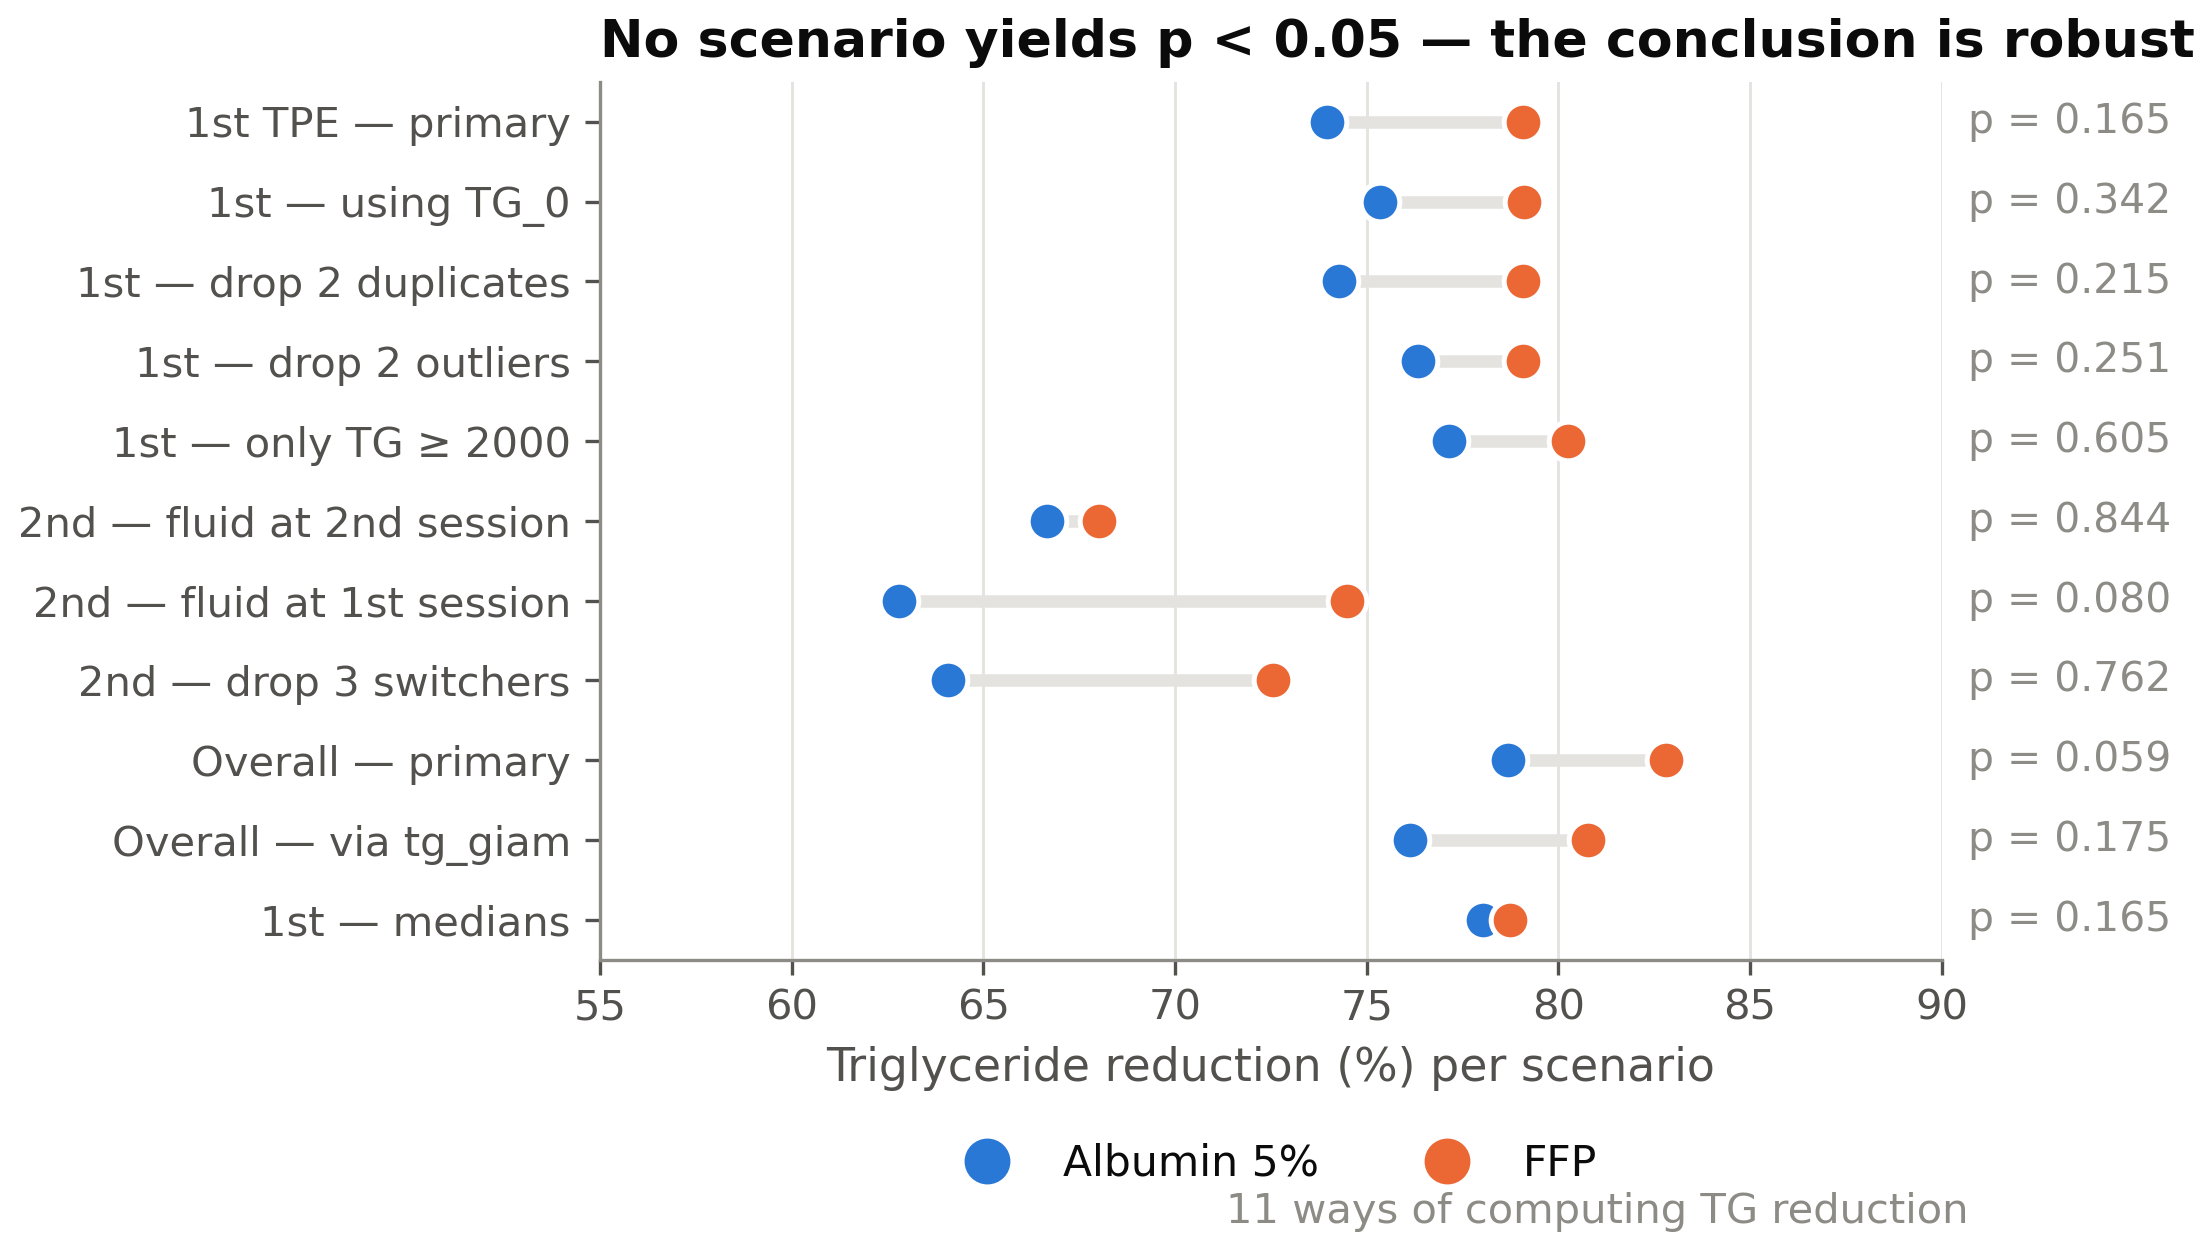
\includegraphics[width=0.86\linewidth]{f10_sensitivity.png}
	}

	\end{poster}

\end{document}
